%%%%%%%%%%%%%%%%%%%%%%%%%%%%%%%%%%%%%%%%%%%%%%%%%%%%
%    Canadian AI Latex Template    %
%%%%%%%%%%%%%%%%%%%%%%%%%%%%%%%%%%%%%%%%%%%%%%%%%%%%
\documentclass[10pt]{cai}

\begin{document}
% Editorial staff will replace the following values:
% 1. Conference Year
% 2. Issue number
% 3. Article DOI
\def\conferenceyear{2025}
\volumeheader{38}{0}%{00.000}
\begin{center}

\title{Efficient and Adversarially Robust Object Detection}
\maketitle

\thispagestyle{empty}

% Add Authors and Affiliations in the camera ready
% for the double blind review, please leave this section as is 
\begin{tabular}{cc}
    Anton Liu\upstairs{\affilone,*}, Roberto Solis-Oba\upstairs{\affilone}
\\[0.25ex]
{\small \upstairs{\affilone} Dept. of Computer Science, Western University} \\
\end{tabular}
  
% Replace with corresponding author email address
\emails{
  \upstairs{*}aliu467@uwo.ca 
}
\vspace*{0.2in}
\end{center}

\begin{abstract}
% This work introduces a novel adaptation of the HYDRA pruning framework to the YOLOv3 object detection model, enhancing both efficiency and adversarial robustness. Deep learning models in safety-critical applications, like autonomous driving, require both computational efficiency and resilience against attacks. We compared structured and unstructured pruning and used DeepLIFT for importance score initialization to assist the pruning. Experimental results show that DeepLIFT-guided unstructured pruning consistently outperforms structured pruning in preserving mean Average Precision (mAP) across pruning levels. This selective pruning maintains robust detection capabilities at high pruning ratios while enhancing real-time processing efficiency.

This work introduces a novel approach to object detection that achieves high efficiency and adversarial robustness by adapting the HYDRA pruning framework to the YOLOv3 model. Object detection deep learning models, particularly in safety-critical applications such as autonomous driving and surveillance, require high computational efficiency and resilience against adversarial attacks. We investigate both structured and unstructured pruning techniques to assess their impact on model size, accuracy, and inference time. By using DeepLIFT for importance scoring we achieve targeted pruning that strikes a balance between model compactness and inference performance. Experimental results show that, when guided by DeepLIFT scoring, unstructured pruning consistently outperforms structured pruning in preserving higher mean Average Precision (mAP) across various pruning levels. DeepLIFT-based importance scoring enables precise pruning, allowing the YOLOv3 model to maintain robust detection performance even at high pruning ratios. This selective pruning method not only reduces computational demands, improving real-time processing capabilities, but also ensures the preservation of critical high detection performance.
\end{abstract}

% add your keywords
\begin{keywords}{Keywords:}
Object Detection, CNN Pruning, Adversarial Robustness, DeepLIFT
\end{keywords}
\copyrightnotice


\section{Introduction}
Object detection is used in numerous real-world applications to enable computers to identify and locate objects within images or videos. Object detection algorithms aim to address two key challenges: determining an object's spatial extent (bounding boxes) and classifying it with the correct label \cite{zhao2019objectdetectiondeeplearning}. These capabilities are cruicial for tasks like autonomous driving, surveillance, and inventory management. Additionally, object detection underpins higher-level vision tasks such as scene understanding and action recognition.

Convolutional Neural Networks (CNNs) have demonstrated remarkable potential for object detection and have been the main subject of recent research \cite{zou2023object}. Designed for processing structured multi-dimensional data like images, CNNs leverage convolutional kernels with learnable weights to detect patterns such as edges, textures, and shapes. Through multiple layers, CNNs construct complex representations, enabling accurate object detection \cite{electronics10202470}.

In safety-critical applications like autonomous driving, failures in object detection systems can have severe consequences, as evidenced by the fatal Uber self-driving car accident in 2018 \cite{Kohli_2019}. While deep learning-based models have improved performance, their vulnerability to adversarial attacks remains a significant challenge \cite{zhang2019adversarially}. Adversarial attacks, which involve maliciously crafted perturbations to input data, can lead to incorrect or missed detections. Adversarial defence aims to enhance model robustness by improving performance under adversarial scenarios, typically through adversarial training \cite{costa2023deep}. 
However, research on defense techniques is limited compared to adversarial attacks, emphasizing the need to enhance model reliability for real-world applications.

Despite their recent success, deep learning methods are computationally intensive during both training and inference due to the need to process large volumes of data through multiple layers. Training requires updating millions of parameters through backpropagation, while inference demands rapid calculations to generate predictions. As models grow in size and complexity, efficiency becomes an increasing concern. Efficiency can be measured in terms of computational resources, such as inference time, memory usage, processing power, and energy consumption \cite{electronics11060945}. 

Several methods can enhance CNN efficiency, including transfer learning, quantization, weight sharing, and pruning \cite{HABIB20224244}. CNN pruning can be either unstructured and structured. Unstructured pruning removes low-contributing weights, creating sparse weight matrices but potentially causing irregular memory access patterns, which can be difficult to optimize on some hardware. Structured pruning, on the other hand, removes entire kernels, resulting in more compact architectures \cite{beforehydra}. Pruning reduces parameters and computational load, making models more suitable for real-time deployment on GPUs or mobile devices.

While adversarial robustness and efficiency have been studied in CNNs, limited research exists that combines these two areas for object detection. This work addresses this by integrating adversarial robustness into efficient object detection frameworks. The main contributions of this work are:

\begin{enumerate}
    \item \textbf{Adaptation of HYDRA for Object Detection:} This work extends HYDRA \cite{hydra}, a robust pruning framework for image classification, to object detection using the YOLOv3 model \cite{redmon2018yolov3incrementalimprovement}. Object detection is more complex than image classification as it requires precise localization along with classification of multiple objects.
    \item \textbf{Evaluation of Pruning Techniques for Object Detection:} We studied structured and unstructured pruning methods to analyze their impact on model size, computational complexity, and mAP performance \cite{iou}. Additionally, we evaluated the performance of pruned models on both colored and greyscale images.
    \item \textbf{Use of DeepLIFT for Importance Scoring:} We integrated the DeepLIFT method to attribute feature contributions to object detection models, enhancing pruning decisions through better initialization.
\end{enumerate}

\section{Background}
\subsection{Object Detection}
\label{secmAP}
Object detection involves classifying and localizing objects within an image or video. For each object, its class, confidence score, and bounding box need to be determined \cite{8627998}. Object detection requires accurate prediction of both the object class and its spatial location, addressing challenges like scale variation, occlusion, and inter-class similarities.

Numerous approaches have been proposed to address object detection challenges. Traditional methods rely on handcrafted features like HOG or Haar-like features with classifiers such as SVM or Random Forests \cite{10099639}, but these methods struggle with complex scenes and scalability. In contrast, convolutional neural networks (CNNs) have significantly improved object detection by learning hierarchical features from raw image data, eliminating manual feature extraction and handling variations in pose, scale, and occlusion. CNNs generalize well across diverse datasets, achieving robustness and good accuracy \cite{cnnvstrad}. 

CNN models for object detection consist of a feature extraction backbone and a detection head for localization and classification. Models like Faster R-CNN \cite{ren2016fasterrcnnrealtimeobject} use a two-stage approach, first generating region proposals and then refining them for classification and localization, while others like the YOLO models \cite{redmon2018yolov3incrementalimprovement} predict bounding boxes and class labels in a single pass. YOLOv3 improves over previous versions of YOLO by using multi-scale detection and a more powerful backbone for better speed and accuracy.


\begin{figure}
    \centering
    \captionsetup{justification=centering}
    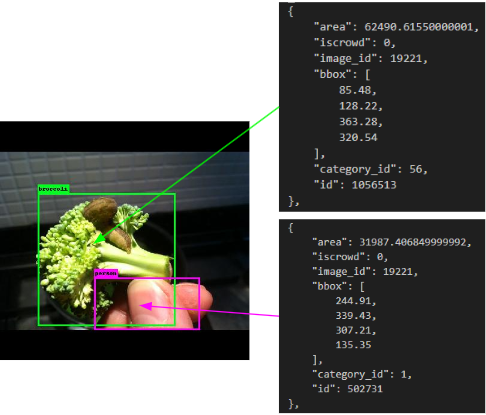
\includegraphics[width=0.5\linewidth]{figs/label.PNG}
    \caption{An example of COCO dataset annotation format}
    \label{fig:coco}
\end{figure}

Datasets are crucial for training object detection models by providing annotated images for model training and evaluation. Existing datasets include Pascal VOC, ImageNet, Open Images \cite{zaidi2021survey}, and MS COCO, one of the most widely used benchmarks \cite{lin2015microsoft}. COCO excels with 80 object classes, including people, animals, vehicles, and household items, ensuring broad generalization. Each image in COCO is annotated with instance-level bounding boxes and class labels, and the dataset includes over 200,000 images for robust training and unbiased evaluation. An example image from COCO is shown in Figure \ref{fig:coco}.

In object detection, mean Average Precision (mAP) is a key metric for evaluating model performance. mAP is the mean of Average Precision (AP) for each class, ranging from 0 to 1, which is derived from the area under the precision-recall curve at various confidence thresholds \cite{map}. Precision is defined as $\frac{\mathrm{TP}}{\mathrm{TP} + \mathrm{FP}}$, and recall is $\frac{\mathrm{TP}}{\mathrm{TP} + \mathrm{FN}}$, where TP, FP, and FN are true positives, false positives, and false negatives, respectively. True positive detections are evaluated using Intersection over Union (IoU) \cite{iou}, which measures the overlap between bounding boxes. mAP is calculated from model outputs at multiple IoU thresholds (0.5 to 0.95) in increments of 0.05 for the COCO dataset, assessing model performance under varying confidence levels. 

In this work, we measure the efficiency of our object detection model by inference time, as it directly impacts real-world performance, especially in real-time or low-latency applications. Inference time indicates how quickly a model can make predictions, which is crucial for time-sensitive tasks like autonomous driving and video-based detection. A model with short inference time can process more data in less time, improving throughput.

\subsection{Adversarial Attack}
Adversarial attacks manipulate neural networks by introducing small, often imperceptible perturbations that cause incorrect predictions \cite{Li_2022}. These attacks expose vulnerabilities in applications like autonomous driving (misclassifying traffic signs), facial recognition (misidentifying individuals), and medical diagnosis (altering disease predictions).

Numerous techniques have been developed to generate adversarial attacks on CNNs, varying in complexity, cost, and effectiveness. The Fast Gradient Sign Method (FGSM) \cite{goodfellow2015explainingharnessingadversarialexamples} is a simple, fast attack that adjusts inputs along the gradient of the loss function. Projected Gradient Descent (PGD) \cite{madry2019deeplearningmodelsresistant} is an iterative method that applies FGSM repeatedly with small steps, creating more robust adversarial examples. The Carlini \& Wagner (C\&W) \cite{carlini2017evaluatingrobustnessneuralnetworks} attack is an optimization-based method known for generating subtle yet effective perturbations.

\subsection{Efficient Adversarial Robustness}
While many studies focus on either improving CNNs' efficiency or robustness to adversarial attacks, few combine both. Vaddadi et al. \cite{EAR1} showcased an efficient CNN model optimized for adversarial robustness, achieving high classification accuracy and effective resistance to adversarial attacks. Another work from Wijayanto et al. \cite{EAR2} explored the vulnerability of CNNs, particularly compressed models used in mobile devices, and investigated methods to enhance their robustness without sacrificing accuracy. Ye et al. \cite{EAR3} presented a framework that combines adversarial training with weight pruning to achieve model compression without sacrificing robustness. Gui et al. \cite{EAR4} introduced an Adversarially Trained Model Compression (ATMC) framework, integrating pruning, factorization, and quantization within a unified optimization structure to achieve compact, adversarially robust models without significant accuracy loss. 

Sehwag et al. \cite{beforehydra} evaluated CNNs' robustness under structured and unstructured pruning, defining a procedure that includes pre-training, weight pruning, and fine-tuning. Their method achieves a 10× compression ratio with 92.5\% robust accuracy on adversarial examples, with unstructured pruning shown to be more effective.

HYDRA, also by Sehwag et al. \cite{hydra}, further enhances CNNs' performance through pruning by integrating robust training objectives with the empirical risk minimization (ERM) framework. In HYDRA, ERM guides pruning by removing less important weights based on minimizing error under adversarial attacks. The robust training objectives aim to improve adversarial resilience, minimizing worst-case loss within a defined perturbation range \cite{mixtrain}. To achieve this, HYDRA utilizes an importance score-based optimization. Scaled initialization initializes scores based on receptive field size, input channels, and weight magnitude, which promotes faster convergence and enhanced performance of SGD compared to random initialization. Extensive experiments on three different datasets and four robust training objectives demonstrate HYDRA's ability to achieve state-of-the-art benign and robust accuracy at high pruning ratios. The HYDRA pipeline can be described in five steps:

\begin{enumerate}
    \item \textbf{Pre-train}: Train the CNN on adversarial examples to minimize a loss objective, formulated by integrating a robust training objective with ERM.
    \item \textbf{Initialize scores}: Assign floating point importance scores to each model weight using scaled initialization.
    \item \textbf{Minimize loss}: Freeze CNN weights and update importance scores during loss minimization. Run predictions using only weights with highest scores, but update all scores through backpropagation.
    \item \textbf{Prune}: Prune less important weights using the frozen importance scores. Create a binary mask to retain the top weights based on their scores.
    \item \textbf{Fine-tune}: Re-train the pruned network with the robust objective to adapt to structural changes and improve performance.
\end{enumerate}

HYDRA was chosen as the foundation for our work due to its strong performance and comprehensive documentation. It secured second place in the auto-attack robustness benchmark \cite{autoattack} and has been cited over 100 times since publication.

Current research on efficient and adversarially robust CNNs often focuses on image classification, a simpler task than object detection. While classification models are easier to prototype and evaluate, they do not address the complexities of object detection, which involves multi-object recognition and localization \cite{10099639}. No research has fully tested these methods on object detection, highlighting a gap in our understanding of their real-world performance, which this work aims to address.


\section{Methodology}
\subsection{Adaptation of HYDRA for Object Detection}
HYDRA was originally developed for image classification, focusing on recognizing and categorizing objects in an image. However, object detection is more complex as it requires not only identifying objects but also localizing them through bounding boxes, highlighting the spatial arrangement of objects within an image. To adapt HYDRA for object detection, we replaced its CNN models with YOLOv3, using weights pre-trained on the COCO dataset to save training time. Several modifications were made to the pruning pipeline to accommodate the object detection framework, ensuring compatibility with YOLOv3's architecture.

First, we restructured HYDRA's dataloader to handle the COCO dataset, which includes multiple object classes and bounding box annotations per image. Annotations were parsed to extract bounding box coordinates, dimensions, and class labels. Images were augmented by padding and resized to 416x416 pixels, ensuring compatibility with YOLOv3's default input size \cite{redmon2018yolov3incrementalimprovement}.

Next, we enhanced output processing. YOLOv3 divides an image into a grid, with each cell predicting multiple bounding boxes, confidence scores, and class probabilities for objects within that cell \cite{redmon2018yolov3incrementalimprovement}. Predictions with confidence scores below 0.5 were filtered out. Then, Non-Maximum Suppression (NMS) \cite{nms} was applied to eliminate redundant bounding boxes, especially when multiple boxes overlap with high IoU, ensuring only the best predictions are retained.

Detection outputs containing image ID, predicted bounding box coordinates, confidence score, and predicted class label are saved in CSV format. mAP performance is calculated using the pycocotools library \cite{lin2015microsoft}, which compares predicted bounding boxes with ground truth annotations at multiple IoU thresholds. The mAP across these thresholds provides a robust measure of YOLOv3’s detection accuracy, capturing performance across various object sizes and overlaps.

Due to the limitations of verifiable robust methods like MixTrain and CROWN-IBP with larger networks, we opted for iterative adversarial training to evaluate robustness. We used mAP as the metric for object detection performance.

\subsection{PGD Attack}
To evaluate the robustness of our model, we used the Projected Gradient Descent (PGD) attack \cite{madry2019deeplearningmodelsresistant}. PGD refines the FGSM method by iteratively applying bounded perturbations in the direction of the gradient. After each step, the perturbation is projected back within a specified range ($\varepsilon$) to maintaining perceptual similarity, using a clip function that trims the changes of pixel values to $\varepsilon$ if they exceed it. PGD’s iterative process make it effective at generating stable adversarial examples, thus serving as the benchmark for evaluating our model's robustness. Figure \ref{fig:dog1} illustrates a PGD attack on an image from the COCO dataset.

Implementing the PGD attack on YOLOv3 generates adversarial perturbations that cause misdetections or missed objects. The algorithm for applying PGD to YOLOv3 is outlined in Algorithm \ref{alg:pgd_attack}. This algorithm ensures that perturbations remain imperceptible to humans while degrading model accuracy.

\begin{algorithm}
    \caption{PGD Attack on YOLOv3 Object Detection}
    \label{alg:pgd_attack}
    \begin{algorithmic}[1]
    \REQUIRE Image $I_0$, model $f$, loss function $\mathcal{L}$, step size $\alpha = 0.02$, bound $\varepsilon = 0.05$, number of steps $n = 5$
    \ENSURE Adversarial image $I'$
    
    \STATE Normalize pixel values of $I_0$ to range $[0, 1]$
    \STATE Initialize adversarial image $I' \gets I_0$
    
    \FOR{$i = 1$ to $n$}
        \STATE Compute gradient: $g \gets \nabla_{I'} \mathcal{L}(f(I'), I_0)$
        \STATE Update image: $I' \gets I' + \alpha \cdot g$
        \STATE Project perturbations: $I' \gets \text{clip}(I', I_0 - \varepsilon, I_0 + \varepsilon)$
    \ENDFOR
    
    \RETURN $I'$
    \end{algorithmic}
\end{algorithm}

\begin{figure}
    \centering
    \captionsetup{justification=centering}
    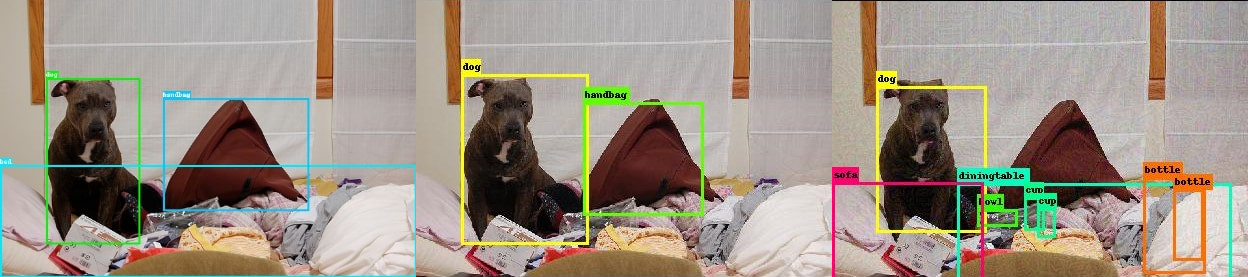
\includegraphics[width=1.0\linewidth]{figs/dog1.jpg}
    \caption{COCO dataset image 22192: Ground truth (left), YOLOv3 on original image (middle), YOLOv3 on PGD perturbed image (right) }
    \label{fig:dog1}
\end{figure}

\subsection{New DeepLIFT Initialization Technique}
The scaled initialization method in HYDRA improves over random initialization for determining parameter weight importance \cite{hydra}. However, other methods could estimate how much each parameter weight contributes to the final output. DeepLIFT (Deep Learning Important FeaTures) \cite{deeplift} is a method that explains neural network outputs by attributing differences in output to changes in input features relative to a defined reference input. It calculates contribution scores for each feature by measuring their impact on the difference of the output from a reference state through specific rules like the RevealCancel rule. The RevealCancel rule is designed to handle situations where positive and negative contributions from inputs interact, potentially cancelling each other out in non-linear layers. By separating and calculating the effects of positive and negative components independently, RevealCancel captures dependencies between inputs that might otherwise be overlooked \cite{deeplift}. This approach offers a more efficient and interpretable means of understanding neural network predictions compared to traditional gradient-based methods, making it ideal for importance score initialization in our pipeline.

The DeepLIFT implementation leverages the Captum library, a model interpretability and understanding library for PyTorch \cite{captum}. We use DeepLIFT to replace step 2 in the original HYDRA pipeline by optimizing importance scores. With DeepLIFT, each weight in the network is assigned an attribution score, a measure of how much it contributes to the model’s final output relative to a reference input. The DeepLIFT scores are used to generate a binary mask that determines which weights or kernels should be pruned, targeting those with minimal contribution to the network. This process replaces traditional importance score initialization for pruning, as the pruning decision is made based on clear, interpretable scores that indicate each weight’s significance.

\subsection{Implementing Unstructured and Structured Pruning}
In addition to the unstructured pruning used in HYDRA, we implemented structured pruning for a comparative analysis. Structured pruning can yield greater reductions in model size and computational complexity while preserving the network's architecture. The comparison highlights the trade-offs between pruning strategies in terms of accuracy, robustness, and efficiency.

We implemented structured pruning by focusing on reducing entire kernels rather than individual weights. Specifically, structured pruning evaluates the importance of each kernel in convolutional layers, and makes pruning decisions at the higher kernel level instead of the lower, more granular weight level. The importance of each kernel is calculated by averaging the importance of all its weights. This means that we  modified the pruning step in the HYDRA pipeline, by applying a binary pruning mask at the kernel level. An additional step is added to process the kernels' importance, and ensure that all the weights inside each kernel have the same value in the binary mask. The mask is a binary tensor that matches the shape of the network's weight tensor, with values indicating whether a weight should be pruned (0) or retained (1).

\section{Experiments}
We conducted experiments with five distinct configurations to evaluate the effects of different pruning strategies and initialization methods. The first four configurations use color COCO images: (1) unstructured pruning with DeepLIFT initialization, (2) unstructured pruning with HYDRA initialization, (3) structured pruning with DeepLIFT initialization, and (4) structured pruning with HYDRA initialization. These configurations allow for a comparison of the performance of the different initialization methods and pruning strategies (Sections \ref{sec1} and \ref{sec2}). The fifth configuration, structured pruning with DeepLIFT initialization, uses COCO images converted to greyscale, enabling a comparison of the method's performance on colored versus greyscale images (Section \ref{sec3}).

For each of the 5 configurations, 10 experimental runs were conducted at each of 9 chosen pruning ratios: 0\%, 25\%, 50\%, 65\%, 75\%, 85\%, 90\%, 95\%, and 99\%, to provide sufficient granularity in the data. Each model was evaluated using pycocotools to calculate the resulting mAP performance, and the average inference time per image was also measured. 

One-way ANOVA (Analysis of Variance) was used to find any statistically significant differences between results. The p-value threshold was set at 0.05, so the null hypothesis is rejected when then p-value is smaller than 0.05. 

A random subset of 50,000 images from the COCO dataset was used for training in the pruning pipeline, while the remaining 150,000+ images were used for testing to evaluate the performance of the pruned model. All experiments were conducted on a NVIDIA GeForce RTX 2070 SUPER GPU.


\subsection{Preliminary Findings}
% describe graph
We present mAP and inference time of different pruning configurations on the testing dataset in Figures \ref{fig:result1} and \ref{fig:result2}. Each curve represents a configuration, showing the average mAP or time across pruning ratios. Averages are calculated by taking the mean of 10 independent runs per pruning ratio, with each run depicted in the figures as a dot. Standard deviations are shown as error bars, reflecting the variability due to the inherent randomness in model training and pruning, as SGD updates are based on randomly selected mini-batches.

% og model
The black dashed lines in the figures represent the performance of the original YOLOv3 model under the same PGD attack, achieving a mAP of 0.176, which is significantly lower than that of models with 0\% pruning. This disparity arises because the latter models undergo additional adversarial pre-training in step 1 of the pipeline, enhancing their resilience. In terms of inference speed, the original model processes an image in 119.3 ms in average, similar to adversarially trained models with no pruning (0\%). This similarity in inference time is due to minimal structural changes, as no weights are removed in either the original or unpruned adversarially trained models, resulting in consistent computational workload.

% performance decrease and pruning increase
Figures \ref{fig:mAP1} and \ref{fig:mAP2} show that the mAP performance of pruned models decreases as the pruning rate increases, due to the removal of increasingly more important parameters that reduce the model's capacity to learn and retain critical information for accurate detection. 

The inference time curve in Figures \ref{fig:time1} and \ref{fig:time2} shows an "S" shape. This is because early pruning stages cause only slight reductions in inference time as few parameters are removed; however, as pruning increases, the network shrinks, leading to a more significant decrease in inference time. Furthermore, beyond a certain threshold, aggressive pruning introduces sparsity, making computation less efficient and causing inference time to plateau due to hardware bottlenecks like memory access.

% object detection harder than classification
In \cite{hydra}, the HYDRA authors focused on pruned performance at 90\%+ pruning rates. However, when adapting HYDRA from image classification to object detection, the performance drop at higher pruning rates (beyond 60\%) is more significant. This is due to the complexity of object detection, which requires detailed spatial and contextual information to detect and localize objects. A more detailed mAP plot for pruning rates 85\%+ is shown in Appendix B Figure 1, where all methods exhibit similar low mAP values \cite{MyAppendix}.

\subsection{DeepLIFT vs Scaled Initialization}
\label{sec1}

\begin{figure}
    \centering
    \captionsetup{justification=centering,margin=1cm}
    \begin{subfigure}[b]{.45\textwidth}
      \centering
      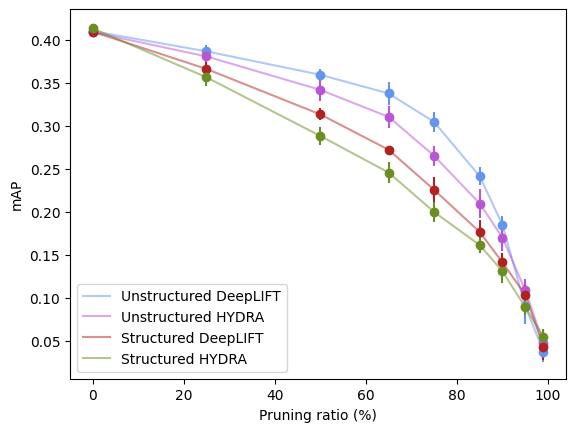
\includegraphics[width=1\linewidth]{figs/mAP1.PNG}
      \caption{mAP}
      \label{fig:mAP1}
    \end{subfigure}%
    \begin{subfigure}[b]{.45\textwidth}
      \centering
      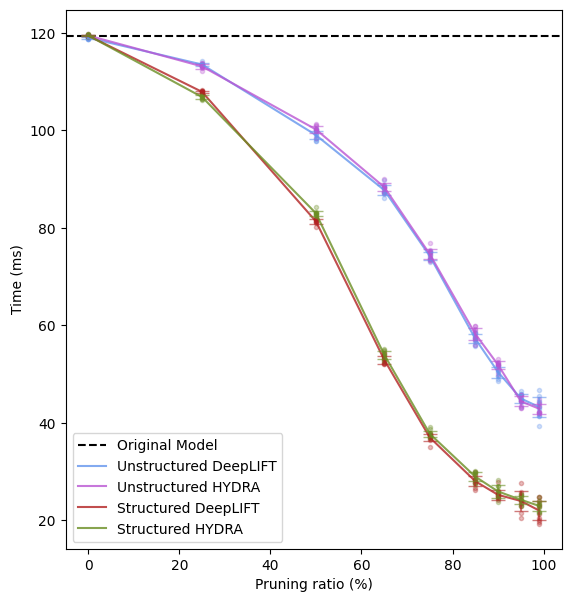
\includegraphics[width=1\linewidth]{figs/time1.PNG}
      \caption{Inference time}
      \label{fig:time1}
    \end{subfigure}
    \caption{Comparison of DeepLIFT versus HYDRA initialized models with both unstructured and structured pruning, through different pruning ratios. A detailed view of the high ratio region is provided in Appendix B  \cite{MyAppendix}.}
    \label{fig:result1}
\end{figure}

% deeplift better
Figure \ref{fig:mAP1} compares mAP performance between models pruned using DeepLIFT versus scaled initialization, DeepLIFT consistently outperforms scaled initialization within the 50\%-85\% pruning ratio range for both pruning methods. This is statistically validated by one-way ANOVA tests, all yielding p-values below the 0.05 threshold, as shown in Appendix B, Table 1 \cite{MyAppendix}. DeepLIFT is more effective than scaled initialization for pruning as it directly calculates each weight's contribution to the final output, unlike scaled initialization, which infers importance partially from weight magnitude.

Scaled initialization overlooks the non-linear relationships between weights and predictions, where large weights may not always be crucial. DeepLIFT, by contrast, provides an attribution score that measures each weight's actual impact on the output, offering a more precise method than size-based importance. DeepLIFT targets weights that truly influence the model, ensuring that the most important components are preserved during pruning. This leads to a more efficient pruned model with higher performance, particularly in a complex task like object detection, where feature and spatial relationships are crucial.

% compare time
When comparing the inference time between pruned models using the two different initialization methods in Figure \ref{fig:time1}, there is no clear difference between the pruning methods. The pruning algorithms aim to reduce the network to a target pruning rate, and inference efficiency primarily depends on the model’s size and structure rather than initial importance scores. ANOVA tests in Table 2 largely support this, with most p-values above 0.05 \cite{MyAppendix}. 

% init time penalty
Using DeepLIFT initialization increases the time to initialize importance scores compared to HYDRA's scaled initialization. Scaled initialization takes an average of 18 seconds, while DeepLIFT requires 49 seconds. DeepLIFT's longer runtime stems from its reference-based approach, which calculates the difference between each neuron's activation and a baseline, a more computationally intensive process than using the magnitude of weights.

\subsection{Unstructured vs Structured Pruning}
\label{sec2}
Figure \ref{fig:mAP1} shows that unstructured pruning consistently outperforms structured pruning in mAP across pruning ratios from 25\% to 90\% for both initialization methods, as supported by the ANOVA p-values in Appendix A, Table 1 \cite{MyAppendix}. Structured pruning typically results in lower mAP due to the removal of entire filters, channels, or layers, which impacts the model’s ability to capture fine-grained features. This is particularly detrimental to object detection tasks that require detailed feature extraction across multiple scales, leading to a more significant performance drop in structured pruning.

While the initialization methods did not have a significant effect on the inference time performance, Figure \ref{fig:time1} shows a significant difference between the two pruning methods. Starting from a 65\% pruning ratio, structured pruned models require about half the time compared to unstructured models at the same pruning ratio. The one-way ANOVA tests in Table 2 support this finding \cite{MyAppendix}. Structured pruning improves inference time by producing an optimized and regularized architecture, with fewer filters or layers and a consistent structure. This enables better memory access patterns and more efficient hardware processing, leading to faster computations, making structured pruning ideal for real-time applications, despite its potential impact on mAP.

\subsection{Effect of Greyscale on Performance}
\label{sec3}
\begin{figure}
    \centering
    \captionsetup{justification=centering}
    \begin{subfigure}[b]{.45\textwidth}
      \centering
      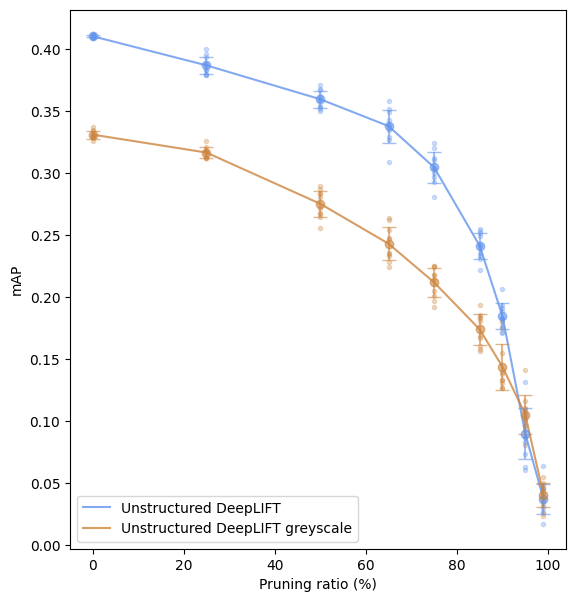
\includegraphics[width=1\linewidth]{figs/mAP2.PNG}
      \caption{mAP}
      \label{fig:mAP2}
    \end{subfigure}%
    \begin{subfigure}[b]{.45\textwidth}
      \centering
      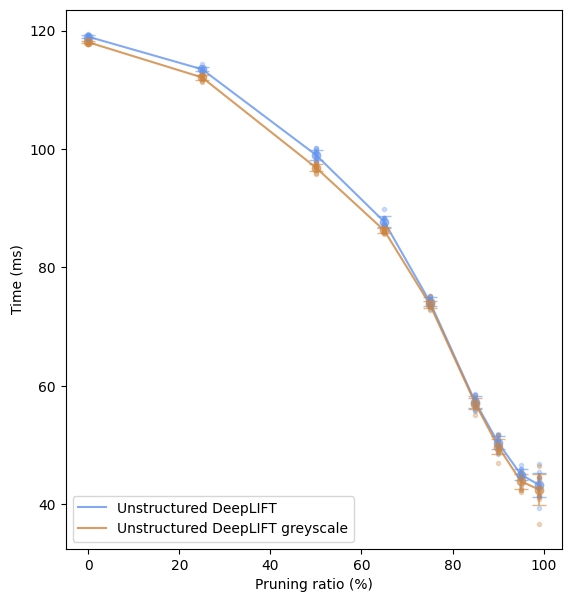
\includegraphics[width=1\linewidth]{figs/time2.PNG}
      \caption{Inference time}
      \label{fig:time2}
    \end{subfigure}
    \caption{Comparison of performance between color and greyscale images on unstructured pruned models initialized with DeepLIFT}
    \label{fig:result2}
\end{figure}

We evaluated the pruning pipeline with greyscale images using the same training images as in previous experiments but converted to greyscale based on the Rec. 601 Standard. For these experiments, we used the unstructured DeepLIFT variant of the pruning pipeline, as it showed the highest mAP performance in earlier tests.

There is little to no difference in inference time performance between the two methods. However, in Figure \ref{fig:mAP2}, models trained with greyscale images exhibit significantly lower mAP compared to those trained with colored images, particularly at lower pruning ratios (0\%-65\%). However, as the pruning ratio increases, the performance gap narrows until the models' performance are indistinguishable at 95\%+ pruning ratios. This stems from the loss of chrominance information in greyscale images. YOLOv3 relies on color to distinguish objects and capture texture, lighting, and shading variations essential for detection. Greyscale images only retain luminance, limiting the model's ability to differentiate objects with similar brightness but different colors. Without color information, it becomes challenging for the model to distinguish between objects like lemons and limes, as both share similar shapes and textures.

\subsection{Sample Images}

\begin{figure}
    \centering
    \captionsetup{justification=centering}
    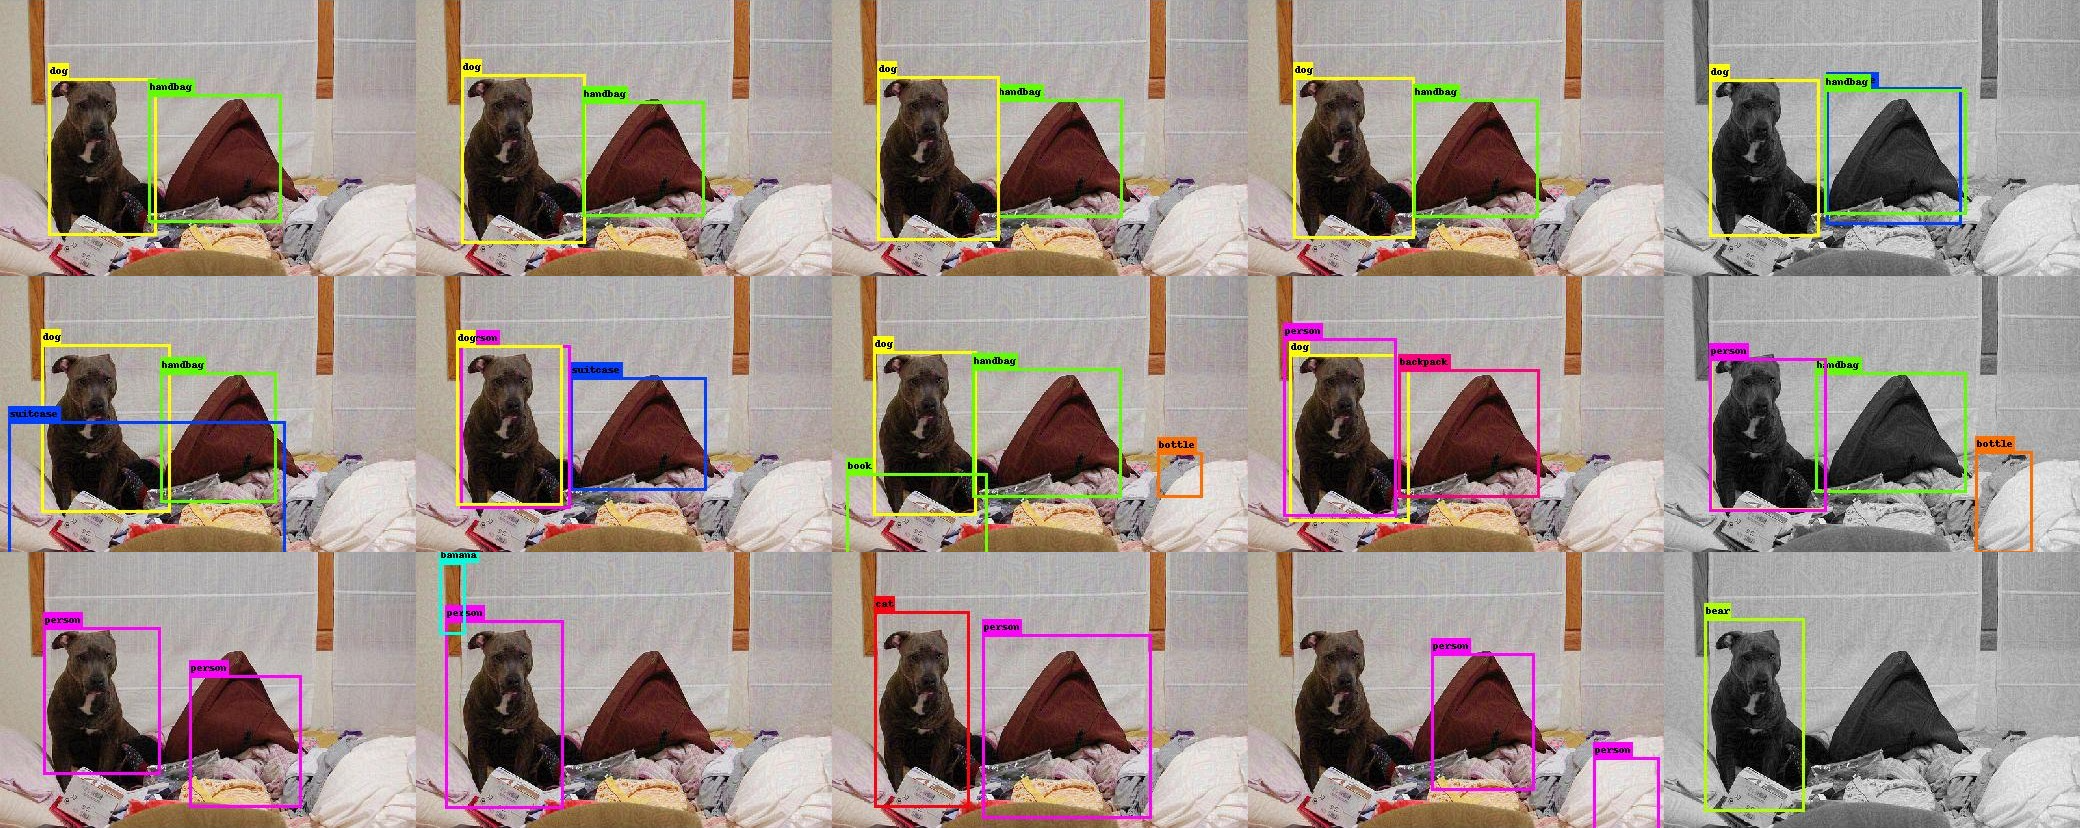
\includegraphics[width=1\linewidth]{figs/22192select.jpg}
    \caption{Differences between inference performance on COCO image 22192: top to bottom pruning ratios - 0\%, 65\%, 95\%; left to right - Unstructured DeepLIFT, Unstructured HYDRA, Structured DeepLIFT, Structured HYDRA, Greyscale Unstructured DeepLIFT.}
    \label{fig:22192select}
\end{figure}

We applied PGD perturbations ($\varepsilon$=0.05) to sample COCO images and performed inference on models trained with different configurations and pruning rates. Appendix B includes the results, where each figure include 45 images across 9 pruning rates and 5 configurations \cite{MyAppendix}. Figure \ref{fig:22192select} shows a subset of examples. Inference was performed on a random model from each of 10 experiment runs, where each detected object is labeled with a colored bounding box and class name.

Visual inspection shows that models pruned on greyscale images perform worse, with fewer correctly detected objects, consistent with mAP results. At low pruning rates (0\% - 25\%), objects are often correctly identified. At high pruning rates (90\% - 99\%), no objects are detected, explaining the mAP drop. At medium pruning rates, unstructured pruning with DeepLIFT initialization consistently outperforms other methods, detecting more objects and reducing misdetections. These observations align with mAP results, confirming DeepLIFT's superiority over HYDRA's scaled initialization.


\section{Conclusions}
This study adapted the HYDRA pruning framework to the YOLOv3 model, enhancing both efficiency and adversarial robustness in object detection. Evaluation between structured and unstructured pruning across various pruning levels revealed that unstructured pruning consistently outperformed structured pruning in preserving higher mean Average Precision (mAP), especially at moderate pruning ratios, thus maintaining good detection accuracy in complex environments. 

Moreover, using DeepLIFT for importance scoring refined the pruning process, targeting parameters with minimal output contribution. This enabled efficient pruning without compromising the model's ability to detect and localize objects accurately, making it suitable for real-time applications like autonomous driving and surveillance.

Future work could explore hybrid pruning techniques that combine structured and unstructured pruning for optimal trade-offs between performance and efficiency. Dynamic pruning ratios, where pruning levels adjust based on a target mAP value, could be useful in real-world deployment. Lastly, testing unstructured pruning with DeepLIFT initialization on models like Faster R-CNN or SSD, with diverse adversarial attacks, and evaluating them on domain-specific datasets, could provide insights into generalizability and adaptability.


% \clearpage
% All references should be stored in the file "references.bib".
% That call to use that file is in "cai.cls". 
% Please do not modify anything below this line.
\printbibliography[heading=subbibintoc]



% \section{Submission Details}
% \label{submission}
% We invite submissions of both long and short papers. Long papers must be no longer than \textbf{12 pages}, and Short papers must be no longer than \textbf{6 pages}, including references, formatted using the conference template. 

% Papers submitted to the conference must contain original work that has not already been published, accepted for publication, or under review by a journal or another conference. Submissions will go through a \textbf{double-blind} review process. Authors are responsible for making sure submissions are anonymized.

% A ``Best Paper Award'' and a ``Best Student Paper Award'' will be given at the conference respectively to the authors of each best paper, as judged by the Best Paper Award Selection Committee.

% \section{Publication and Registration}
% \label{pub}
% Since 2020, the conference proceedings are published through PubPub open access\footnote{\url{https://www.pubpub.org/}} and indexed DBLP, ACM, Google Scholar, and other services that access Pubpub publications.

% At least one author of each accepted paper is required to attend the conference to present the work. The authors must agree to this requirement prior to submitting their paper for review.

% In addition, the corresponding author of each paper, acting on behalf of all of the authors of that paper, must complete and sign a Consent-to-Publish form. The corresponding author signing the copyright form should match the corresponding author marked on the paper.

% \section{Figures and Tables}

% This simple \LaTeX\xspace template has been tested with \texttt{latex} and with \texttt{pdflatex} commands, directly from the command line or through \texttt{latexmk}. We ask that you place captions below tables and figures as in the examples below.

% Pubpub uses a fairly complete \LaTeX\xspace engine that is likely to handle your source files without problems. Please check \url{https://help.pubpub.org/pub/latex-compatibility} if you require specialized packages or non-standard customization.

% \begin{figure}[ht]
%   \centering
%   \ifpdf
%     
\includegraphics[scale=0.6]{figs/sample_fig.png}
%   \else
%     
\includegraphics[scale=0.6,natwidth=330,natheight=120]{figs/sample_fig.png}
%   \fi
%   \caption{Captions under figures, please.}
%   \label{fig:sample_fig}
% \end{figure}

% \begin{table}[h]
% \begin{tabular}{|l|l|}
% \textbf{Header one} & \textbf{Header two} \\ 
% \hline
%  Some text & More text
% \end{tabular}
% \vspace{0.2cm}
% \caption{Captions under tables, please.}
% \label{tab:important}
% \end{table}

% \section*{Acknowledgements}
% This section can be left blank during double-blind review. 


%Appendixes go here
% \appendix

% \clearpage
% \section{ANOVA test results}
% \label{appendix:anova}

% \begin{table}[htbp]
%     \begin{center}
%     \begin{tabular}{ |p{3.3cm}|p{0.6cm}|p{0.6cm}|p{0.6cm}|p{0.6cm}|p{0.6cm}|p{0.6cm}|p{0.6cm}|p{0.6cm}|p{0.6cm}|  }
%      \hline
%      Pruning ratio  & 0\% & 25\%& 50\%& 65\%& 75\%& 85\%& 90\%& 95\%& 99\%\\
%      \hline
%      DeepLIFT vs. HYDRA (Unstructured)    & 1.03 e-01& 9.53 e-02& 1.71 e-03& 3.60 e-04& 1.57 e-06& 1.64 e-04& 2.43 e-02& 3.54 e-02& 1.86 e-01 \\
%      \hline
%      DeepLIFT vs. HYDRA (Structured)     & 1.48 e-02& 3.60 e-02& 1.18 e-05& 1.24 e-05& 6.91 e-04& 1.17 e-02& 8.99 e-02& 8.87 e-03& 5.80 e-02\\
%      \hline
%      Unstructured vs. Structured (DeepLIFT)      & 6.52 e-01& 2.35 e-05& 3.70 e-11& 4.25 e-11&4.20 e-10& 1.13 e-09& 5.46 e-08& 1.09 e-01&3.99 e-01 \\
%      \hline
%      Unstructured vs. Structured (HYDRA)    & 9.00 e-04& 1.11 e-05& 1.17 e-08& 3.05 e-09&4.44 e-10& 6.27 e-07& 1.80 e-05& 1.83 e-03&2.42 e-01\\
%     %  \hline
%     %  Greyscale       & 1.13e-23& 1.74e-15& 1.06e-13& 1.18e-11& 2.53e-12& 2.77e-& 1.75e-05& 9.25e-02& 5.06e-01 \\
%      \hline
%     \end{tabular}
%     \end{center}
    
%     \caption{ANOVA test p-values of mAP on colored COCO images}
%     \label{tab:p-mAP}
% \end{table}

% \begin{table}[htbp]
%     \begin{center}
%     \begin{tabular}{ |p{3.3cm}|p{0.6cm}|p{0.6cm}|p{0.6cm}|p{0.6cm}|p{0.6cm}|p{0.6cm}|p{0.6cm}|p{0.6cm}|p{0.6cm}|  }
%      \hline
%      Pruning ratio  & 0\% & 25\%& 50\%& 65\%& 75\%& 85\%& 90\%& 95\%& 99\%\\
%      \hline
%      DeepLIFT vs. HYDRA (Unstructured)    & 1.28 e-05& 5.61 e-02& 7.16 e-03& 1.44 e-01& 3.96 e-01& 7.69 e-02& 4.37 e-03& 2.05 e-01& 6.64 e-01 \\
%      \hline
%      DeepLIFT vs. HYDRA (Structured)     & 5.13 e-01& 1.81 e-06& 2.80 e-06& 1.37 e-02& 4.21 e-02& 6.36 e-02& 2.06 e-01& 7.33 e-01& 2.15 e-01\\
%      \hline
%      Unstructured vs. Structured (DeepLIFT)      & 1.75 e-04& 4.13 e-19& 4.31 e-21& 1.07 e-24& 2.76 e-26& 2.02 e-22& 6.17 e-21& 1.85 e-16& 1.68 e-14 \\
%      \hline
%      Unstructured vs. Structured (HYDRA)    & 8.70 e-01& 2.76 e-17& 1.03 e-21& 8.97 e-26& 3.45 e-25& 1.30 e-21& 3.55 e-21& 2.36 e-20& 1.56 e-19\\
%     %  \hline
%     %  Greyscale       & 6.11e-09& 2.07e-07& 1.14e-05& 4.42e-04& 2.08e-01& 5.59e-01& 2.62e-01& 3.98e-02& 4.82e-01 \\
%      \hline
%     \end{tabular}
%     \end{center}
%     \caption{ANOVA test p-values of inference time on colored COCO images}
%     \label{tab:p-time}
% \end{table}

% \begin{table}[htbp]
%     \begin{center}
%     \begin{tabular}{ |p{3.3cm}|p{0.6cm}|p{0.6cm}|p{0.6cm}|p{0.6cm}|p{0.6cm}|p{0.6cm}|p{0.6cm}|p{0.6cm}|p{0.6cm}|  }
%     \hline
%     Pruning ratio  & 0\% & 25\%& 50\%& 65\%& 75\%& 85\%& 90\%& 95\%& 99\%\\
%      \hline
%      Greyscale vs color (Unstructured DeepLIFT)      & 1.13 e-23& 1.74 e-15& 1.06 e-13& 1.18 e-11& 2.53 e-12& 2.77 e-10& 1.75 e-05& 9.25 e-02& 5.06 e-01 \\
%      \hline
%     \end{tabular}
%     \end{center}
%     \caption{ANOVA test p-values of mAP on greyscale COCO images}
%     \label{tab:p2-mAP}
% \end{table}

% \begin{table}[htbp]
%     \begin{center}
%     \begin{tabular}{ |p{3.3cm}|p{0.6cm}|p{0.6cm}|p{0.6cm}|p{0.6cm}|p{0.6cm}|p{0.6cm}|p{0.6cm}|p{0.6cm}|p{0.6cm}|  }
%      \hline
%      Pruning ratio  & 0\% & 25\%& 50\%& 65\%& 75\%& 85\%& 90\%& 95\%& 99\%\\
%      \hline
%      Greyscale vs color (Unstructured DeepLIFT)       & 6.11 e-09& 2.07 e-07& 1.14 e-05& 4.42 e-04& 2.08 e-01& 5.59 e-01& 2.62 e-01& 3.98 e-02& 4.82 e-01 \\
%      \hline
%     \end{tabular}
%     \end{center}
%     \caption{ANOVA test p-values of inference time on greyscale COCO images}
%     \label{tab:p2-time}
% \end{table}

% \clearpage
% \section{Figures}
% \label{appendix:figures}

% \begin{figure}[H]
%     \centering
%     \captionsetup{justification=centering}
%     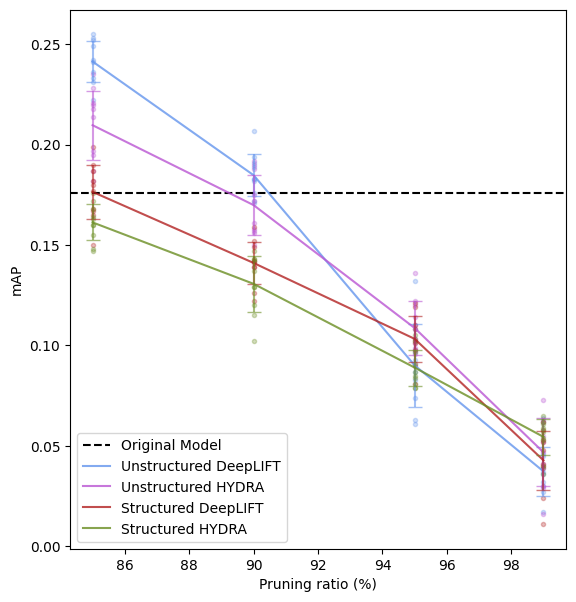
\includegraphics[width=0.5\linewidth]{figs/mAP1zoom.png}
%     \caption{Zoomed in high pruning ratio section of Fig. \ref{fig:mAP1}}
%     \label{fig:mAP1zoom}
% \end{figure}

% \begin{figure}
%     \centering
%     \captionsetup{justification=centering}
%     \includegraphics[width=1.0\linewidth]{figs/attackALLcrop.jpg}
%     \caption{Differences between inference performance on COCO image 22192: pruning ratio increases from top to bottom (0\%, 25\%, 50\%, 65\%, 75\%, 85\%, 90\%, 95\%, 99\% ); experiment configuration changes from left to right (Unstructured DeepLIFT, Unstructured HYDRA, Structured DeepLIFT, Structured HYDRA, Grey Unstructured DeepLIFT). Images below are set up in the same order}
%     \label{fig:attackAll}
% \end{figure}

% \begin{figure}
%     \centering
%     \captionsetup{justification=centering}
%     \includegraphics[width=0.95\linewidth]{figs/17627.jpg}
%     \caption{Differences between inference performance on the COCO image 17627}
%     \label{fig:sample2}
% \end{figure}

% \begin{figure}
%     \centering
%     \captionsetup{justification=centering}
%     \includegraphics[width=0.95\linewidth]{figs/19221.jpg}
%     \caption{Differences between inference performance on the COCO image 19221}
%     \label{fig:sample3}
% \end{figure}

% \begin{figure}
%     \centering
%     \captionsetup{justification=centering}
%     \includegraphics[width=0.95\linewidth]{figs/71711.jpg}
%     \caption{Differences between inference performance on the COCO image 71711}
%     \label{fig:sample4}
% \end{figure}

% \begin{figure}
%     \centering
%     \captionsetup{justification=centering}
%     \includegraphics[width=0.95\linewidth]{figs/174482.jpg}
%     \caption{Differences between inference performance on the COCO image 174482}
%     \label{fig:sample5}
% \end{figure}

% \clearpage
% % All references should be stored in the file "references.bib".
% % That call to use that file is in "cai.cls". 
% % Please do not modify anything below this line.
% \printbibliography[heading=subbibintoc]

\end{document}
